\section{Theoretical Analysis}
\label{sec:analysis}

For the theoretical simulation, we used the dependent voltage source model of the transistors, with Bf1=178.7 and Bf2=227.3.

The bias circuit, which is constituted by $V_c$, $R_{B1}$ and $R_{B2}$, will determine $V_b$.

To simplify the bias circuit, we can ignore the capacitors and make a Thevenin equivalent. This yields:

\begin{equation}
	R_B=\frac{R_{B1} R_{B2}}{R_{B1}+R_{B2}}
\end{equation}

\begin{equation}
	V_{eq}= \frac{R_{B2}}{R_{B1}+R_{B2}} V_{c}
\end{equation}

To calculate the current that passes through the node 8 we know that $I_E= (1+\beta_f)I_B$.

The mesh equation for the bias circuit is $V_{eq} + R_BI_B + V_{Beon} + R_EI_E =0$

Substituting the equation of $I_E$, we now have an expression for $I_B$:
\begin{equation}
	I_{B}= \frac{V_{eq}-V_{ON}}{R_{B}+(1+\beta_F)R_{E}}
\end{equation}

The equation for $I_C$, which is the current that passes trough node 2, is simply $I_C = \beta_F I_B$.

Then, looking at the other mesh, constituted by $R_E, Q_1, R_C$ and$ V_c$, we have the equation:
\begin{equation}
	V_{o}= V_c-R_{C}I_{C}
\end{equation}

By Ohm's Law we also know that $V_E= R_EI_E$ so the voltage between $R_C$ and $R_E$ is: $V_{CE} = V_o - V_E$


We now have all the static voltages and cuurents computed.

For the results of the OP analysis we obtain:

\begin{table}[H]
    \addtolength{\tabcolsep}{-4pt}
    \caption{Some values of the operating point analysis}
    \vspace{-3mm}
    \begin{tabular}{|c|c|}
    \hline
    I_{b1} &  5.0044e-05\\
    I_{e1} &  0.0089929\\
    I_{c1} &  0.0089429  \\ 
    V_{CE1} &  2.1578\\
    I_{b2} &  3.610556e-04 \\
    I_{e2} &  0.082429\\
    I_{c2} &  0.082068\\
    V_{CE2} & 4.4858\\
    \hline
    \end{tabular}
    \label{tab:OP_mat}
\end{table}

The incremental model of the transistor was used to calculate the input and output impedances, as well as
the gain on both stages of the circuit. The capacitors were modelled as short circuits in this stage. This yields:

\begin{table}[H]
    \addtolength{\tabcolsep}{-4pt}
    \caption{SGains and Impedances}
    \vspace{-3mm}
    \begin{tabular}{|c|c|}
    \hline
    Z_{i1} &  484.43\\
    Z_{o1} &  886.28\\
    Z_{i2} &  8598.9\\
    Z_{o2} &  0.30217\\
    Gain_1 & -262.79\\
    Gain_2 &  0.99195\\
    Gain_{Total} & -260.67\\   
    \hline
    \end{tabular}
    \label{tab:Z_mat}
\end{table}

Lastly, the capacitors were re-introduced in order to calculate the gain as a function of the frequency after each stage.
The results are graphed below:

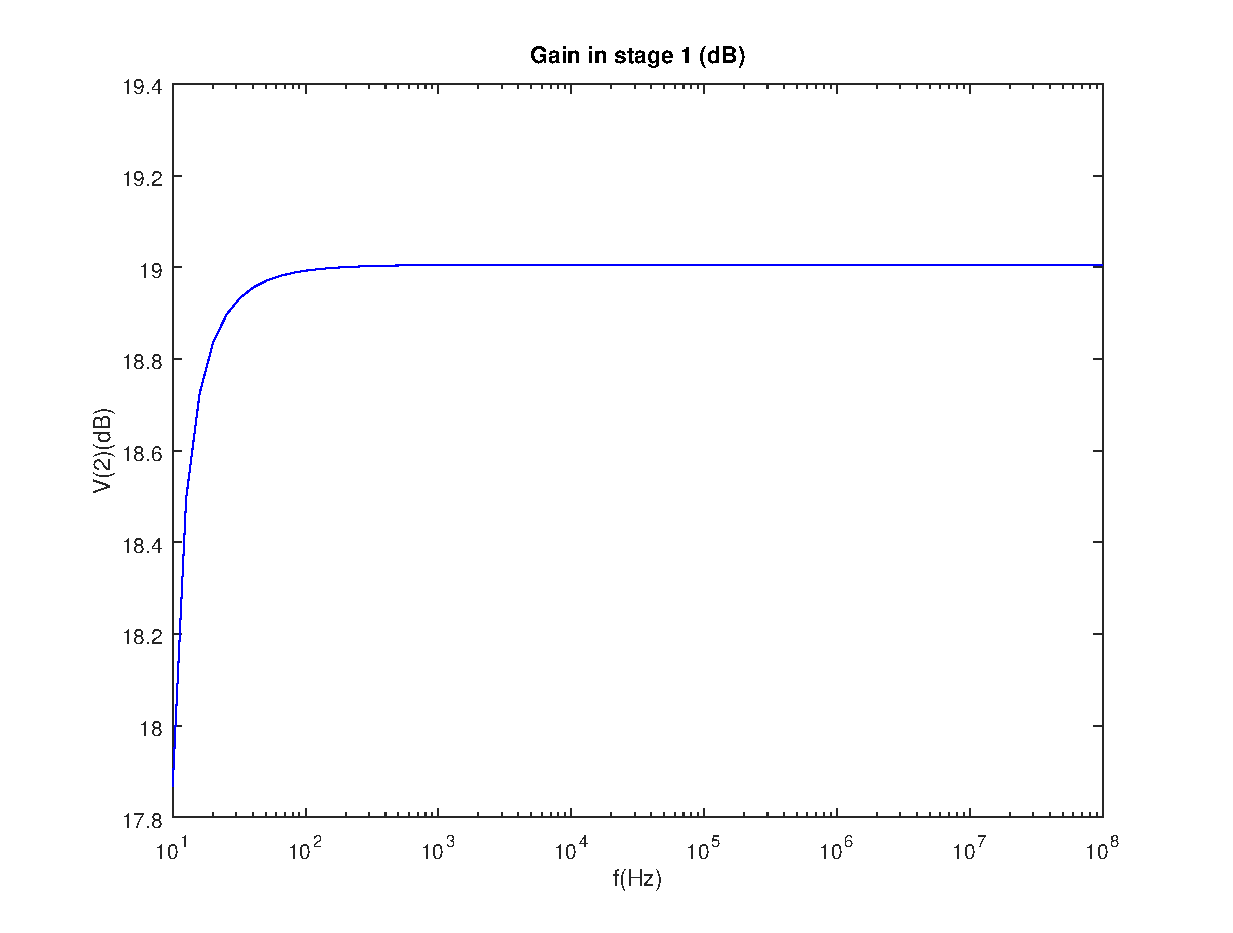
\includegraphics[width=1\linewidth]{vo1.eps}

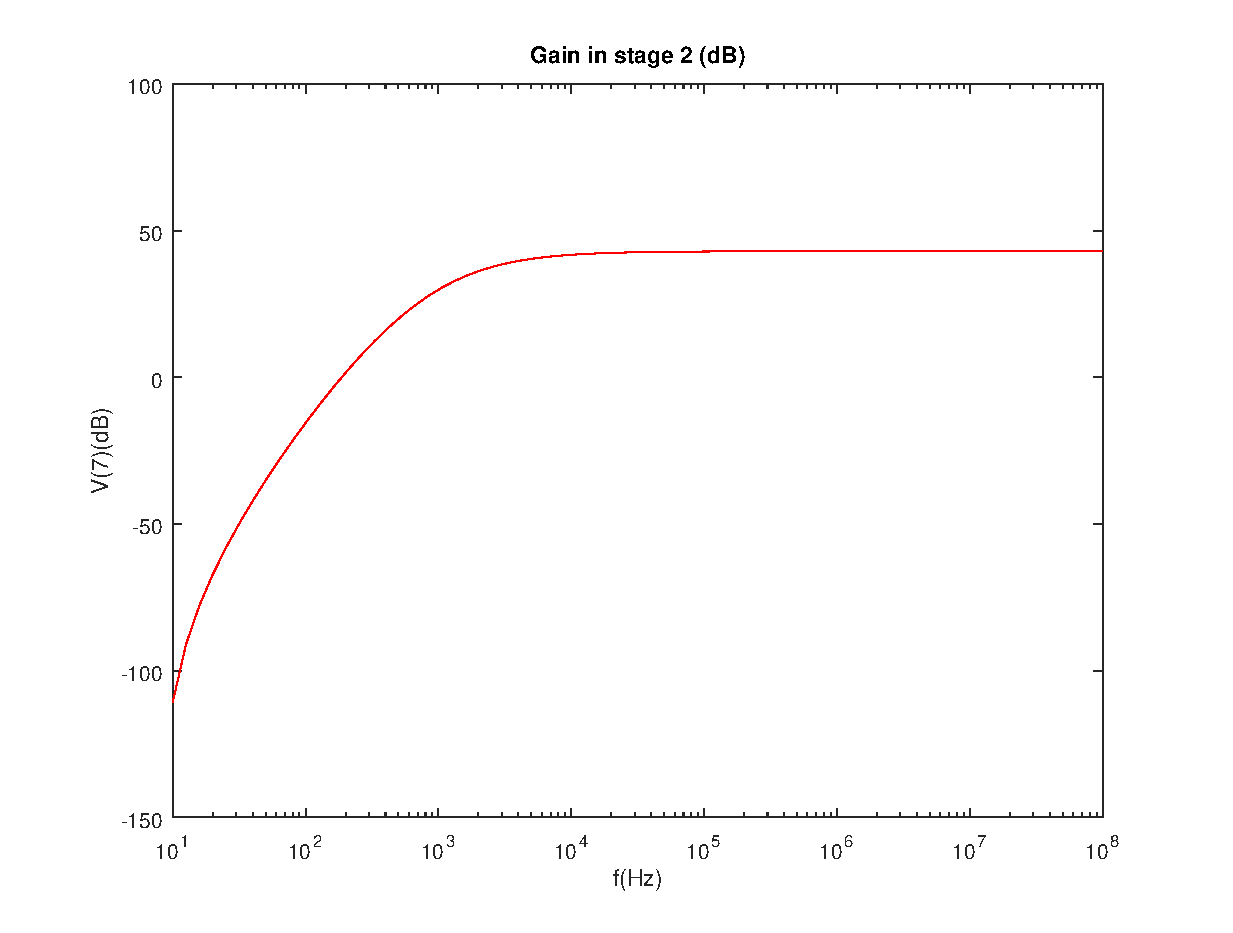
\includegraphics[width=1\linewidth]{vo2.eps}

The lower 3dB cut-off point is at $f=5484.4 Hz$
As we can see, the lower cut-off point is accurrate, but this model does not deal well with the higher cut-off point.
